 \documentclass[11pt]{article}

\usepackage{latexsym}
\usepackage{amssymb}
\usepackage{amsthm}
\usepackage{amscd}
\usepackage{amsmath}
\usepackage{tikz}
\usepackage{graphicx}
\usepackage{enumerate}

\newcommand{\ZZ}{\mathbb{Z}}

\setlength{\evensidemargin}{1in}
\addtolength{\evensidemargin}{-1in}
\setlength{\oddsidemargin}{1.5in}
\addtolength{\oddsidemargin}{-1.5in}
\setlength{\topmargin}{1in}
\addtolength{\topmargin}{-1.5in}

\setlength{\textwidth}{16cm}
\setlength{\textheight}{23cm}

\newcommand{\rook}{\hspace{-.1cm}\amalg\hspace{-.15cm}\bar{}}
\newcommand{\Stab}{\mathrm{Stab}}
\newcommand{\FF}{\mathbb{F}}


\begin{document}
\begin{center}
\section*{William Daniels}
\section*{CSCI 4630}
\subsection*{Linguistic Geometry}
\subsection*{Homework \#6 03/08/15}
\end{center}

\vspace{.25cm}

The primary effect of this change would be it becomes harder \and harder to generate higher-level negations, since you are always forcing the pieces to be able to negate in the smallest amount of time possible. To make this clear, we'll look at the second negation generated in class. The board with the specified main trajectory is shown below: \\\\
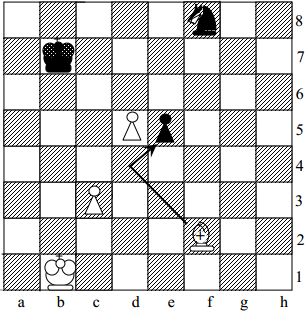
\includegraphics{2ndNegation.png}\\\\

Now, the zone normally looks like:
$$ t(BISHOP, t_B, 3)t(King, t_K, 3)t((KNIGHT, t_K), 2)t(WPAWN, t_WP, 2)t((BPAWN, t_BP), 2)t((WPAWN, t_WP), 3)t(KNIGHT, t_K, 3)t(WPAWN, 2)$$
This is because the amount of time it'll take the king to move along the first negation is higher than the white pawn moving along the second negation. The same applies to the black knight, which, although it normally takes him only 2 moves to get to the negation trajectory, taking the maximum makes it so that he has a time of 3 to reach the pawn and create the 2nd negation. \\
Now, if we change the ALPHA function as specified (taking the minimum instead of the maximum), when we are creating the 2nd negation trajectory, we use the shortest time to the negation trajectory. For example, our zone would turn into:
$$ t(BISHOP, t_B, 3)t(King, t_K, 3)t((KNIGHT, t_K), 2)t(WPAWN, t_WP, 1)t((BPAWN, t_BP), 2)t((WPAWN, t_WP), 3)t(KNIGHT, t_K, 2)t(WPAWN, 1)$$
This is interesting, because we are considering the negation trajectories, which are essentially ``helping'' trajectories, it much more accurately models what we actually want to accomplish. This makes it so that there is no ``extra time'' represented throughout the trajectory, and for an opposing piece to create an even higher negation trajectory, they would have much less time to accomplish that! A good example would be if there was an additional white knight located at H7. Normally, in order to be able to produce a negation trajectory for this piece, you would need to take three moves. Now, with our original definition of the zones, this would be a valid negation trajectory! as the final location had a time of ``3'' assigned to it. However, with the modified ``ALPHA'' function, it becomes obvious that the white knight has no chance of creating a negation, since it has no way of reaching the negation location in a time of ``2''. This is a very simple example of the impact, but the gist of it is that it results in a large reduction of negation trajectories, which models a much closer-to-reality zone which takes into account the fact that many pieces are done negating earlier than the previous definition of the ALPHA function.






\end{document}

